\documentclass[11pt]{article}

% --- Page layout ---
\usepackage[a4paper,margin=2cm]{geometry}

% --- Typography and section formatting ---
\usepackage{titlesec}
\titleformat{\section}{\normalfont\Large\bfseries}{}{0pt}{}
\titleformat{\subsection}{\normalfont\large\bfseries}{}{0pt}{}
\usepackage{parskip}

% --- Figures and tables ---
\usepackage{graphicx}
\usepackage{float}
\usepackage{booktabs}
\usepackage{caption}
\usepackage{subcaption}
\captionsetup[figure]{justification=centering}
\usepackage{url}

% --- Citations ---
\usepackage{endnotes}
\let\footnote=\endnote
\usepackage{bibentry}
\nobibliography*

% --- Document starts here ---
\begin{document}
	
	\begin{center}
		\LARGE\textbf{Ship Detection Pipeline for Smart Port Monitoring}
	\end{center}
	
	\section*{Introduction}
	
	Can pre-trained CNN models accurately detect ships in satellite images to support smart port operations?

	Background and Related Works
	
	Deep learning has become a powerful tool for detecting ships in optical satellite images, significantly advancing maritime surveillance\endnote{\bibentry{patel2022}}
	
	Discuss why detecting ships via satellite imagery benefits smart ports
	- Real-time identification of vessels in port areas can support traffic management, berth allocation, and security
	- Also complements Automatic Identification System (AIS) data by catching ships that might not broadcast their location
	
	Recent work has focus on object detection networks like YOLO for ship localisation\endnote{\bibentry{patel2022}}
	Others have used sliding-window classifiers on satellite images\endnote{\bibentry{rhammell2017}}
	2023 review by Zhao et al. discusses challenges of small object (ship)detection in high-resolution imagery, and various CNN-based solutions\endnote{\bibentry{zhao2024}}
	
	Mention a little bit about the data when introducing the overall workflow of this project
	
	Clearly defined research question: this report investigates whether pre-trained convolutional neural networks can be fine-tuned to detect ships in satellite imagery of ports, with smart port applications in mind.
	
	\newpage
	\section*{Data and Methods}
	
	We are using the ShipsNet dataset (4000 labelled image chips from Planet satellite imagery) and how it was originally created
	Consists of 4,000 RGB image chips (80 * 80 pixels at 3m resolution) extracted from Planet Scope scene over San Francisco Bay and San Pedro Bay. Each chip is labelled as 'ship' (1) or 'no-ship' (0). Mention that 
	The dataset curator ensured the "no-ship" class includes challenging false targets like partial ships and linear features that fooled models
	Be sure to cite the source of the dataset (Kaggle) https://www.kaggle.com/datasets/rhammell/ships-in-satellite-imagery
	
	Note the class distribution before balancing: "The original dataset contains 1000 'ship' chips and 3000 'no-ship' chips (no actual ship present, partial ship, or look-alike structure), which will be relevant when discussing errors
	
	to avoid data leakage, we first stratified the original dataset into 80\% training and 20\% test sets. We then performed class balancing only on the training set by upsampling the minority "ship" class to match the number of "no-ship" samples. The test set was kept with its natural class imbalance to ensure an unbiased evaluation of model performance.
	
	Data Preparation: we performed class balancing by upsampling the minority class ('ship') - generated additional 'ship' samples by random resampling to match the number of no-ship images
	Why? balancing prevents the model from simply always predicting the majority class.
	Potential pitfall - since we performed upsampling before splitting into train/test, there is a slight risk that duplicate ship chips could appear in both sets
	To avoid and chance of train/test leakage, a best practice is to first split the original data, then augment or upsample only the training set (this will be addressed prior to the write-up)
	
	Data Augmentation: We used horizontal and vertical flips on training images (50\% probability each) to account for different orientations of ships. Additional augmentations include small rotations up to plus minus 20 degrees (since ships appear at arbitrary angles), colour jitter - brightness, contrast and saturation tweaks (to simulate different lighting or water conditions in satellite imagery) After augmentation, all images were resized to 224*224 pixels to match the input size expected by the pre-trained models, converted to floating point, and normalised using the ImageNet mean and standard deviation values.
	
	Use of Pre-Trained Models: describe the models and transfer learning strategy we used. We fine-tuned three ImageNet-pretrained CNN architectures - VGG11, ResNet50, and EfficientNet-B0, for binary classification. We tried multiple architectures for comparison. For each model, we customised the final layer to output 2 classes (ship vs no-ship). We leveraged transfor learning by freezing the early layers. so only the new classifier layer trains. This approach, known as feature extraction, is effective with limited data because it uses the pre-trained convolutional laers as fixed feature detectors. We opted to freeze the base convolutional layers to avoid overfitting, given only ~3.200 training chips after augmentation.
	
	Training Procedure: Summarising how we trained the models. 80\% train, 20\% test, stratified. Note key hyperparameters - we used the Adam optimizer with learning rate = 5e-4 and trained for 30 epochs (why?). Adam is a popular optimiser for deep learning tasks because it combined adaptive learning rates with momentum, making it suitable for fast and stable convergence, especially with transfer learning and small datasets. 5e-4 is a reasonable moderate starting learning rate for fine-tuning: low enough to avoid "blowing up" the pretrained weights, but high enough to still allow reasonably fast convergence. Keeping early convolutional layers frozen prevents overfitting and reduces training time. Early stopping was not explicitly applied
	
	Evaluation Metrics: mention that during training we monitored accuracy and loss on both training and test sets each epoch. After training, we evaluated the models on the test set using metrics like overall accuracy, precision, recall, and a confusion matrix. We'll present a table of results for the three models.
	
	We'll be adding a pipeline diagram to the report (flowchart format)
	
	Ship Detection: After training the classifier, we tackled object detection in larger port images - We applied the trained classifier to detect ships in full satellite scenes via a sliding-window approach. We slide a 80*80 pixel window across the image (with some stride) Each window is classified by the model as ship or no-ship. If the model predicts 'ship' with high confidence, you record that window's location as a detection. Because a single ship will result in many neighbouring windows all classified as ship, we then apply Non-Maximum Suppression (NMS) to merge overlapping window hits into one final bounding box per ship. We set a confidence threshold of 0/95 for predictions and an IoU threshold of 0.1 for NMS (confidence threshold filters out low-probability detections; NMS with IoU 0.1 means any overlapping detections are merged if they shared >10\% area)
	
	Mention application of Captum for model interpretability - we performed occlusion-based attribution to see which parts of an image influence the model's prediction. We slid a 20*20 mask over test images to compute occlusion importance maps, helping verify that the model focuses on the ship pixels when classifying an image as 'ship'. Explainable AI literature.
	
	\begin{figure}[H]
		\centering
		\caption{Class Samples (\textit{ship} and \textit{no-ship})}
		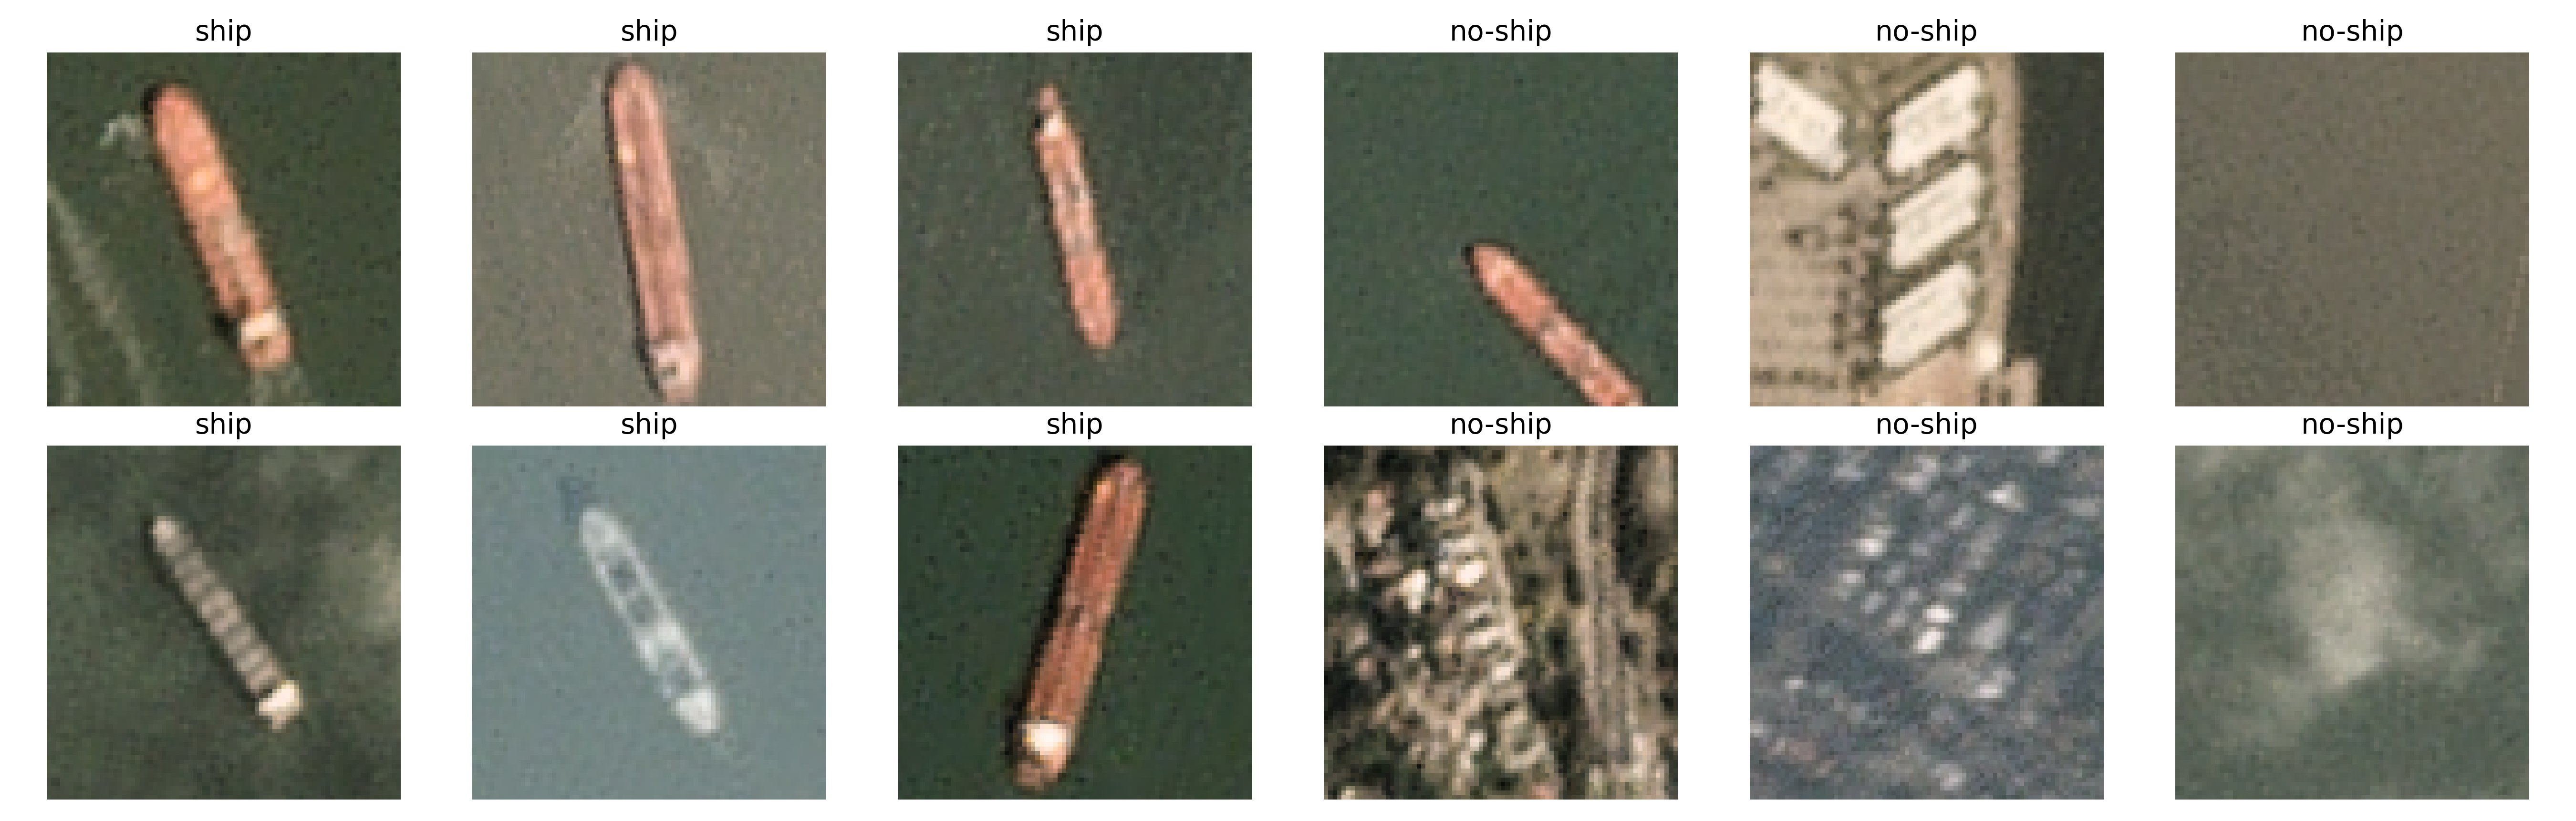
\includegraphics[width=\linewidth]{assets/data_example/ship_vs_noship_examples.png}
	\end{figure}
	
	\section*{Results and Discussion}
	
	\begin{figure}[H]
		\centering
		\caption{Evaluation Results}
		
		% Table of performance metrics
		\begin{subfigure}[b]{0.95\textwidth}
			\centering
			\makebox[\textwidth]{
			\renewcommand{\arraystretch}{1.5}
			\small
			\begin{tabular}{lccccccc}
				\specialrule{1.2pt}{0pt}{0pt}
				\textbf{Model} & \textbf{Accuracy} & \textbf{Precision} & \textbf{Recall} & \textbf{F1 Score} & \textbf{Best Epoch} & \textbf{Train Loss} & \textbf{Test Loss} \\
				\midrule
				VGG11            & 0.9500 & 0.9200 & 0.9400 & 0.9300 & 24/30 & 0.2147 & 0.1361 \\
				\midrule
				ResNet50         & 0.9200 & 0.8800 & 0.9200 & 0.9000 & 11/30 & 0.1981 & 0.1900 \\
				\midrule
				EfficientNet-B0  & 0.8800 & 0.8300 & 0.9000 & 0.8500 & 13/30 & 0.2357 & 0.2644 \\
				\specialrule{1.2pt}{0pt}{0pt}
			\end{tabular}
			}
			\vspace{0.75em}
			\caption{Performance Metrics and Losses at Best Epoch}
		\end{subfigure}
		
		\vspace{1em}
		
		\setcounter{subfigure}{1}
		
		% Confusion Matrices
		\begin{subfigure}[b]{\textwidth}
			\centering
			\begin{subfigure}[b]{0.32\textwidth}
				\centering
				\captionsetup{labelformat=empty}
				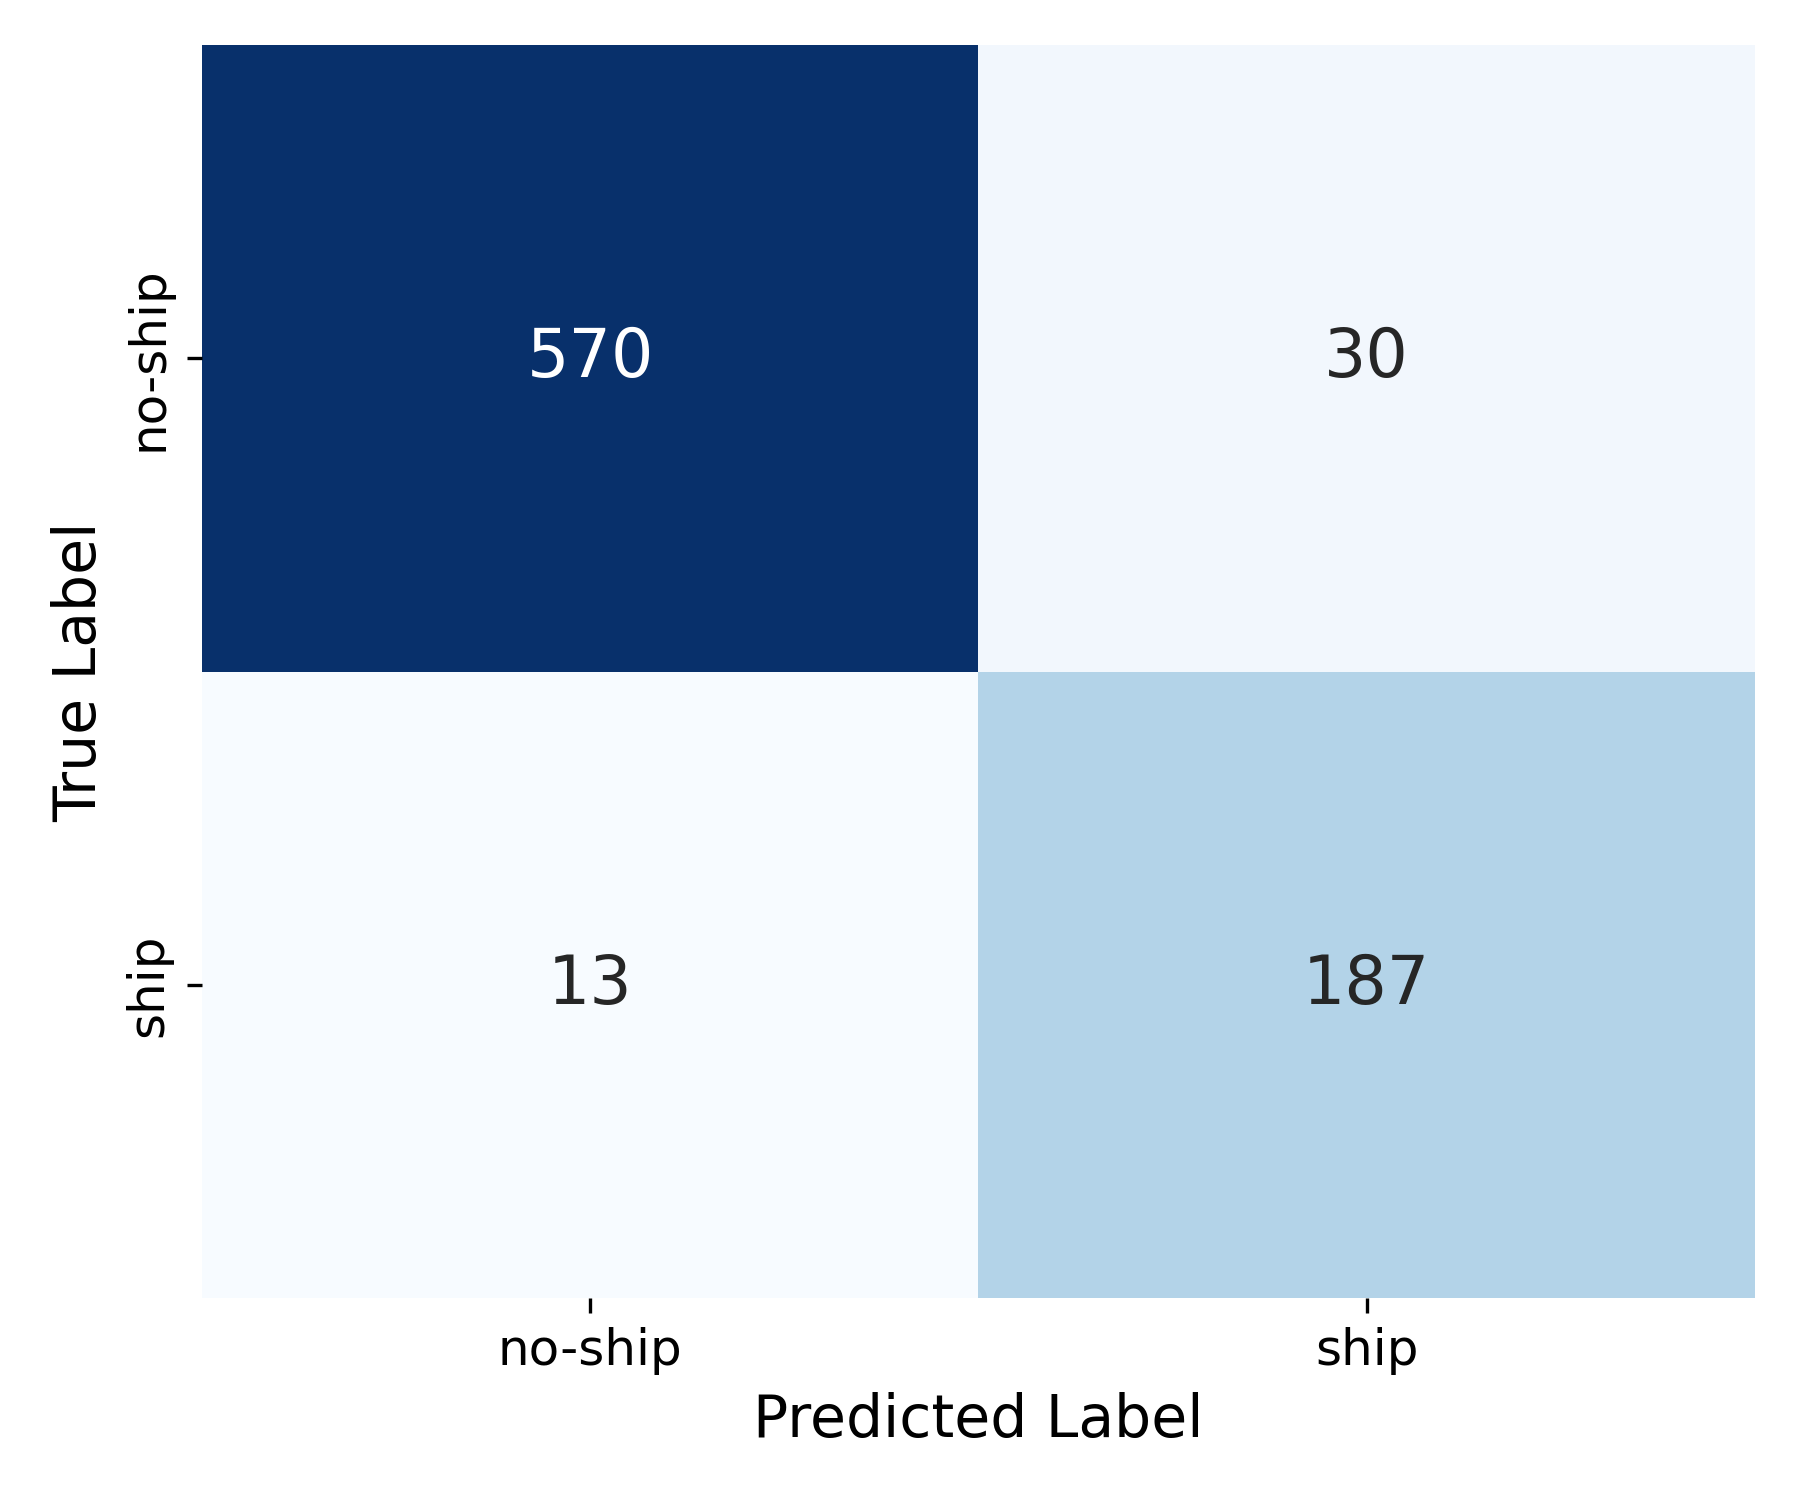
\includegraphics[width=\textwidth]{assets/confusion_matrix/vgg11_confusion_matrix.png}
				\caption*{1. VGG11}
			\end{subfigure}
			\hfill
			\begin{subfigure}[b]{0.32\textwidth}
				\centering
				\captionsetup{labelformat=empty}
				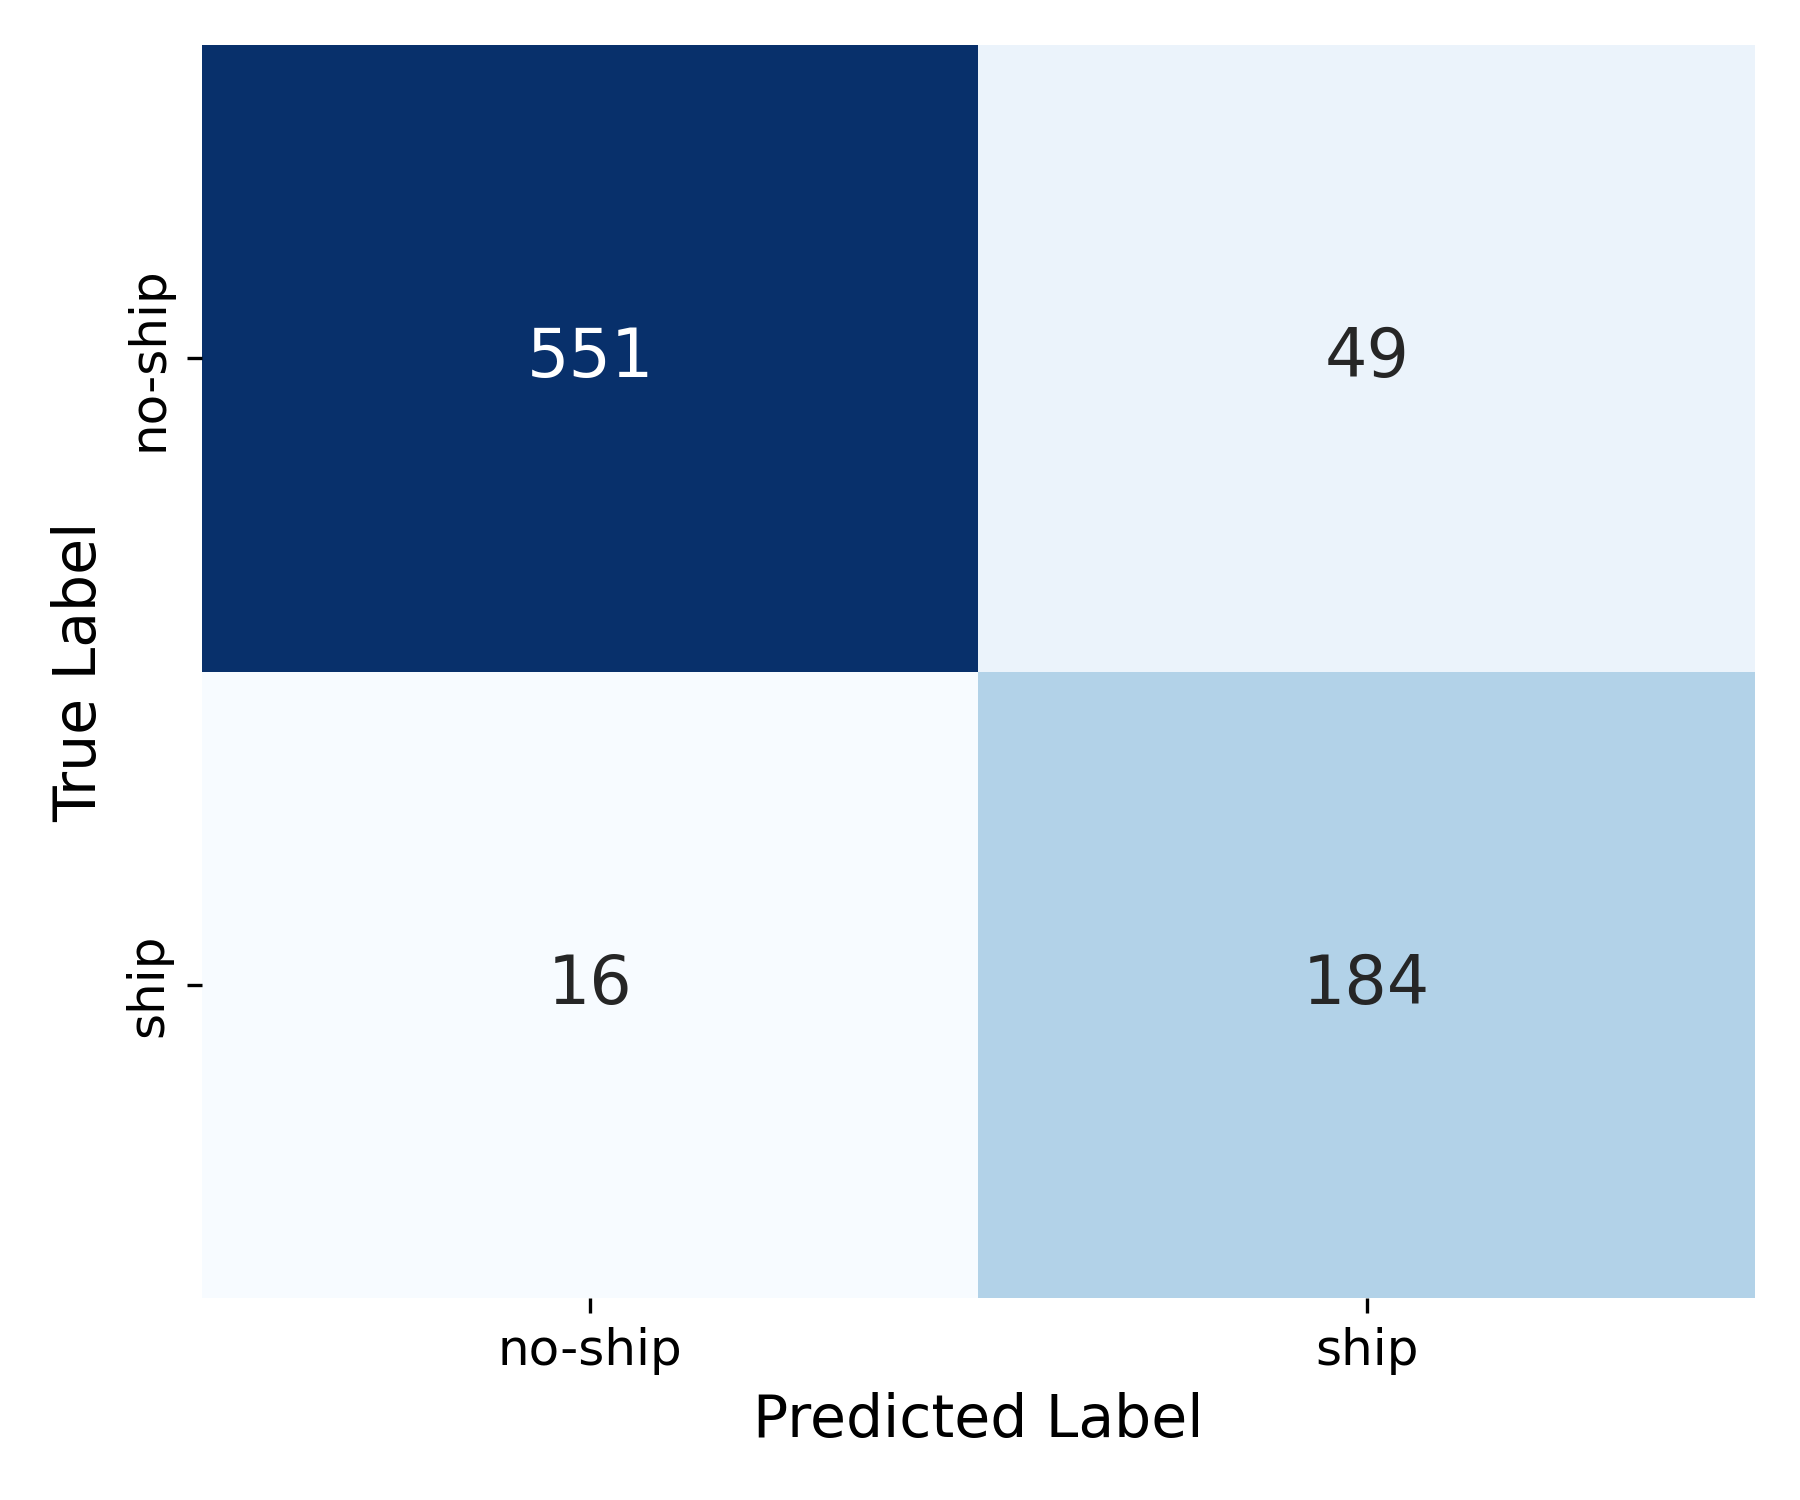
\includegraphics[width=\textwidth]{assets/confusion_matrix/resnet50_confusion_matrix.png}
				\caption*{2. ResNet50}
			\end{subfigure}
			\hfill
			\begin{subfigure}[b]{0.32\textwidth}
				\centering
				\captionsetup{labelformat=empty}
				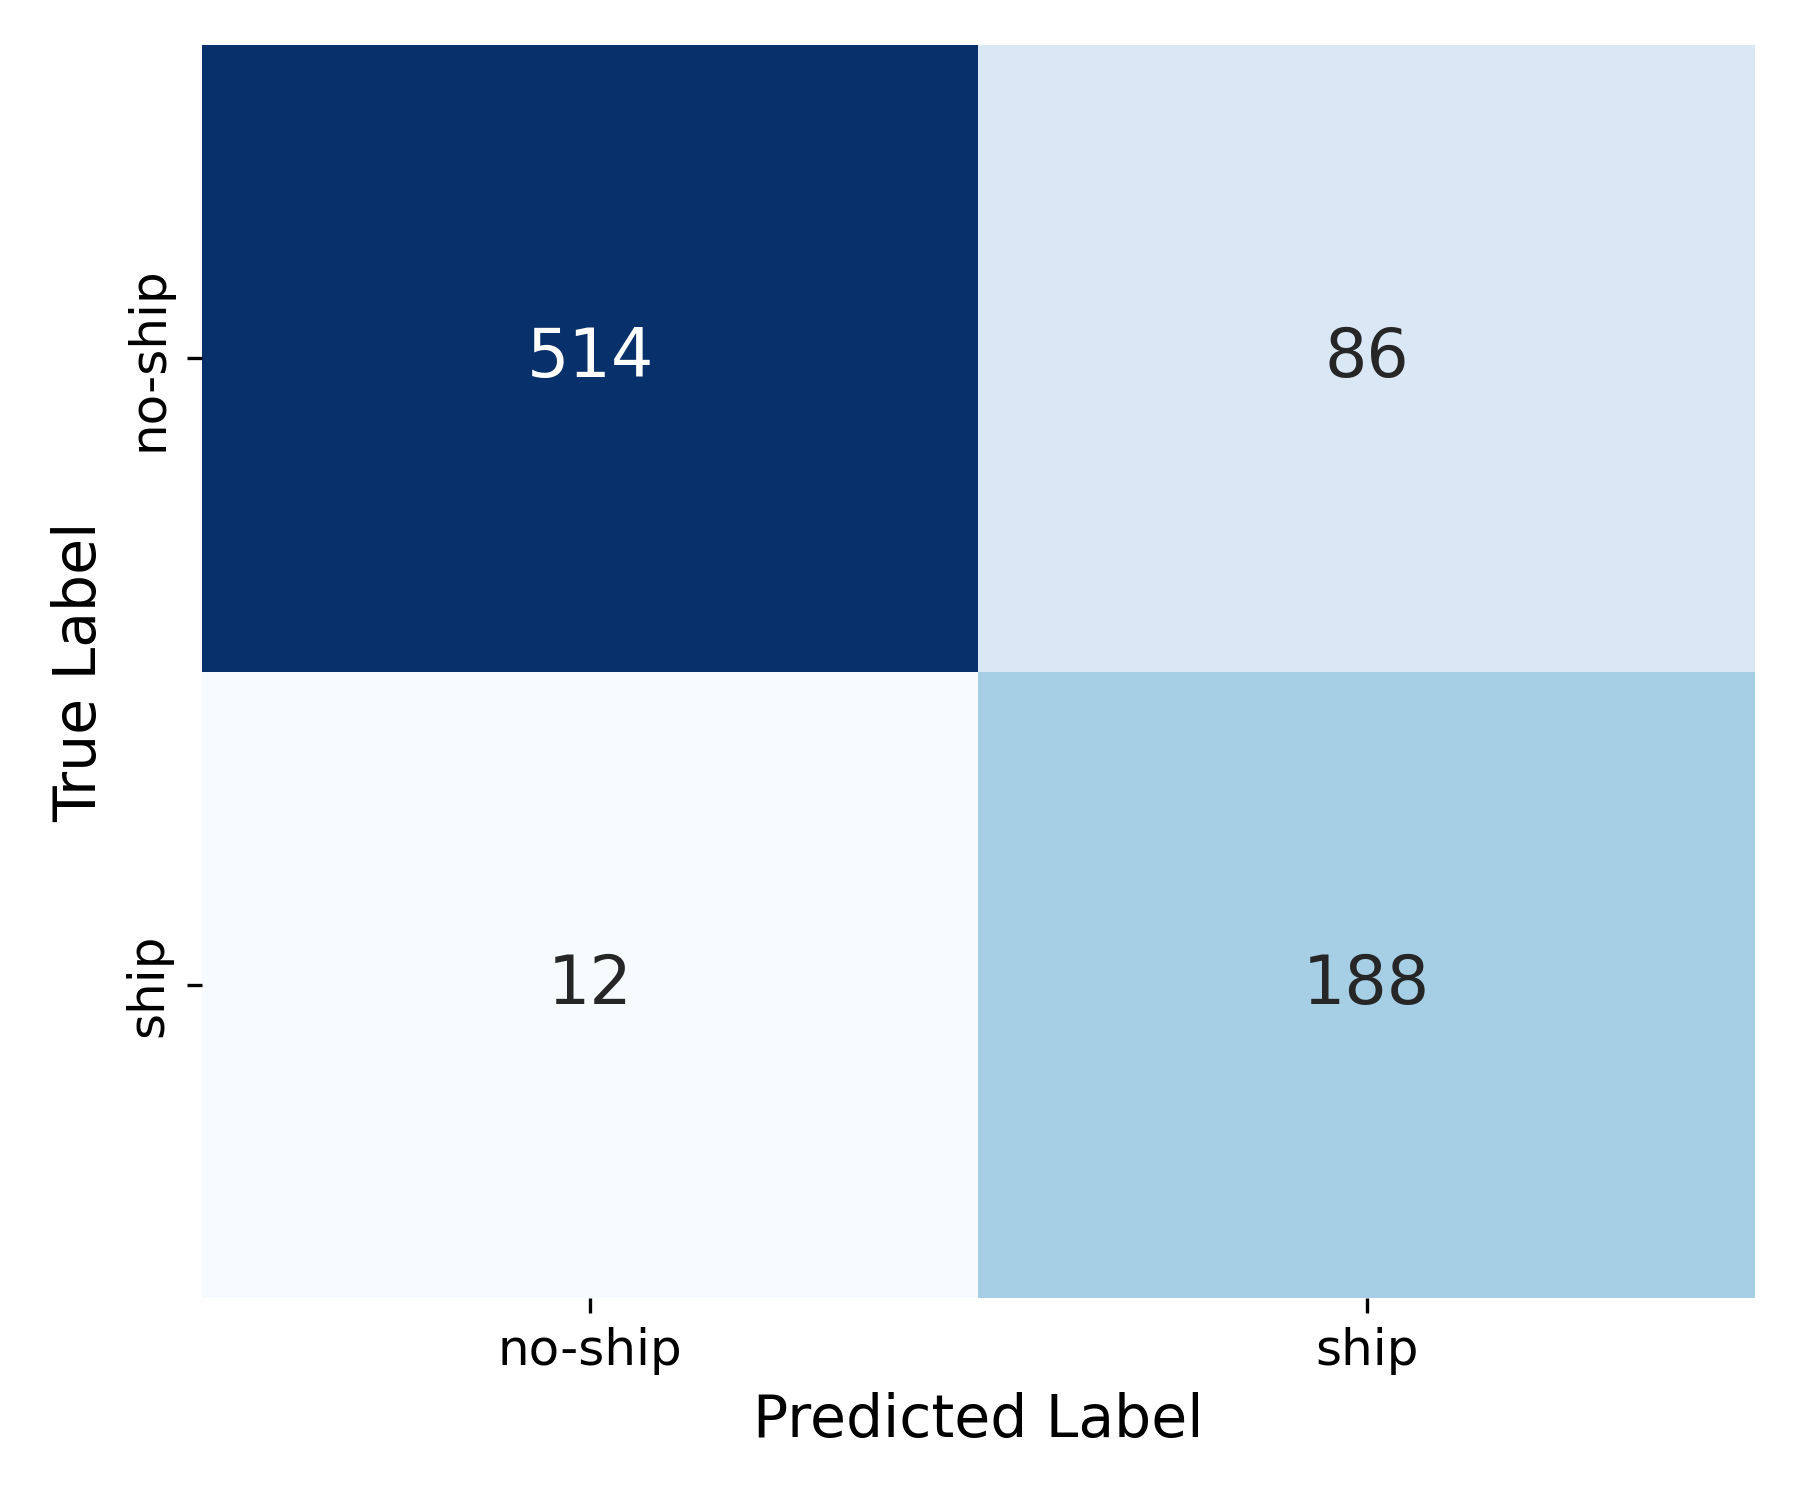
\includegraphics[width=\textwidth]{assets/confusion_matrix/efficientnet_confusion_matrix.png}
				\caption*{3. EfficientNet-B0}
			\end{subfigure}
			\caption{Confusion Matrices}
		\end{subfigure}
		
	\end{figure}
	
	Among the three fine-tuned models evaluated—VGG11, ResNet50, and EfficientNet-B0—VGG11 achieved the highest overall performance, with an accuracy of 95\%, precision of 92\%, recall of 94\%, and an F1 score of 93\%, reaching optimal performance after 29 epochs. The high recall and balanced precision suggest that VGG11 was particularly effective in detecting ships with minimal false negatives, which is critical in maritime surveillance applications. ResNet50 also demonstrated strong performance, achieving a 92\% accuracy, 88\% precision, 92\% recall, and a 90\% F1 score, with earlier convergence at 16 epochs. While slightly less precise than VGG11, ResNet50's faster convergence and comparably high recall indicate it may offer a good trade-off between detection quality and training efficiency, particularly when computational resources are limited. EfficientNet-B0, despite achieving the fastest convergence at 18 epochs, lagged slightly behind with an accuracy of 88\%, precision of 83\%, recall of 90\%, and an F1 score of 85\%. Its lower precision indicates a higher rate of false positives, suggesting that while it is computationally efficient and lightweight, it may not be the optimal choice where high precision is critical. Overall, VGG11 offered the best balance between precision and recall, while ResNet50 provided a strong alternative with faster training. EfficientNet-B0, although attractive for deployment scenarios with strict resource constraints, showed a performance drop that may limit its use in applications demanding high detection reliability.
	
	
%q	% Sample Predictions
%	\begin{subfigure}[b]{0.95\textwidth}
%		\centering
%		\begin{subfigure}[b]{0.32\textwidth}
%			\centering
%			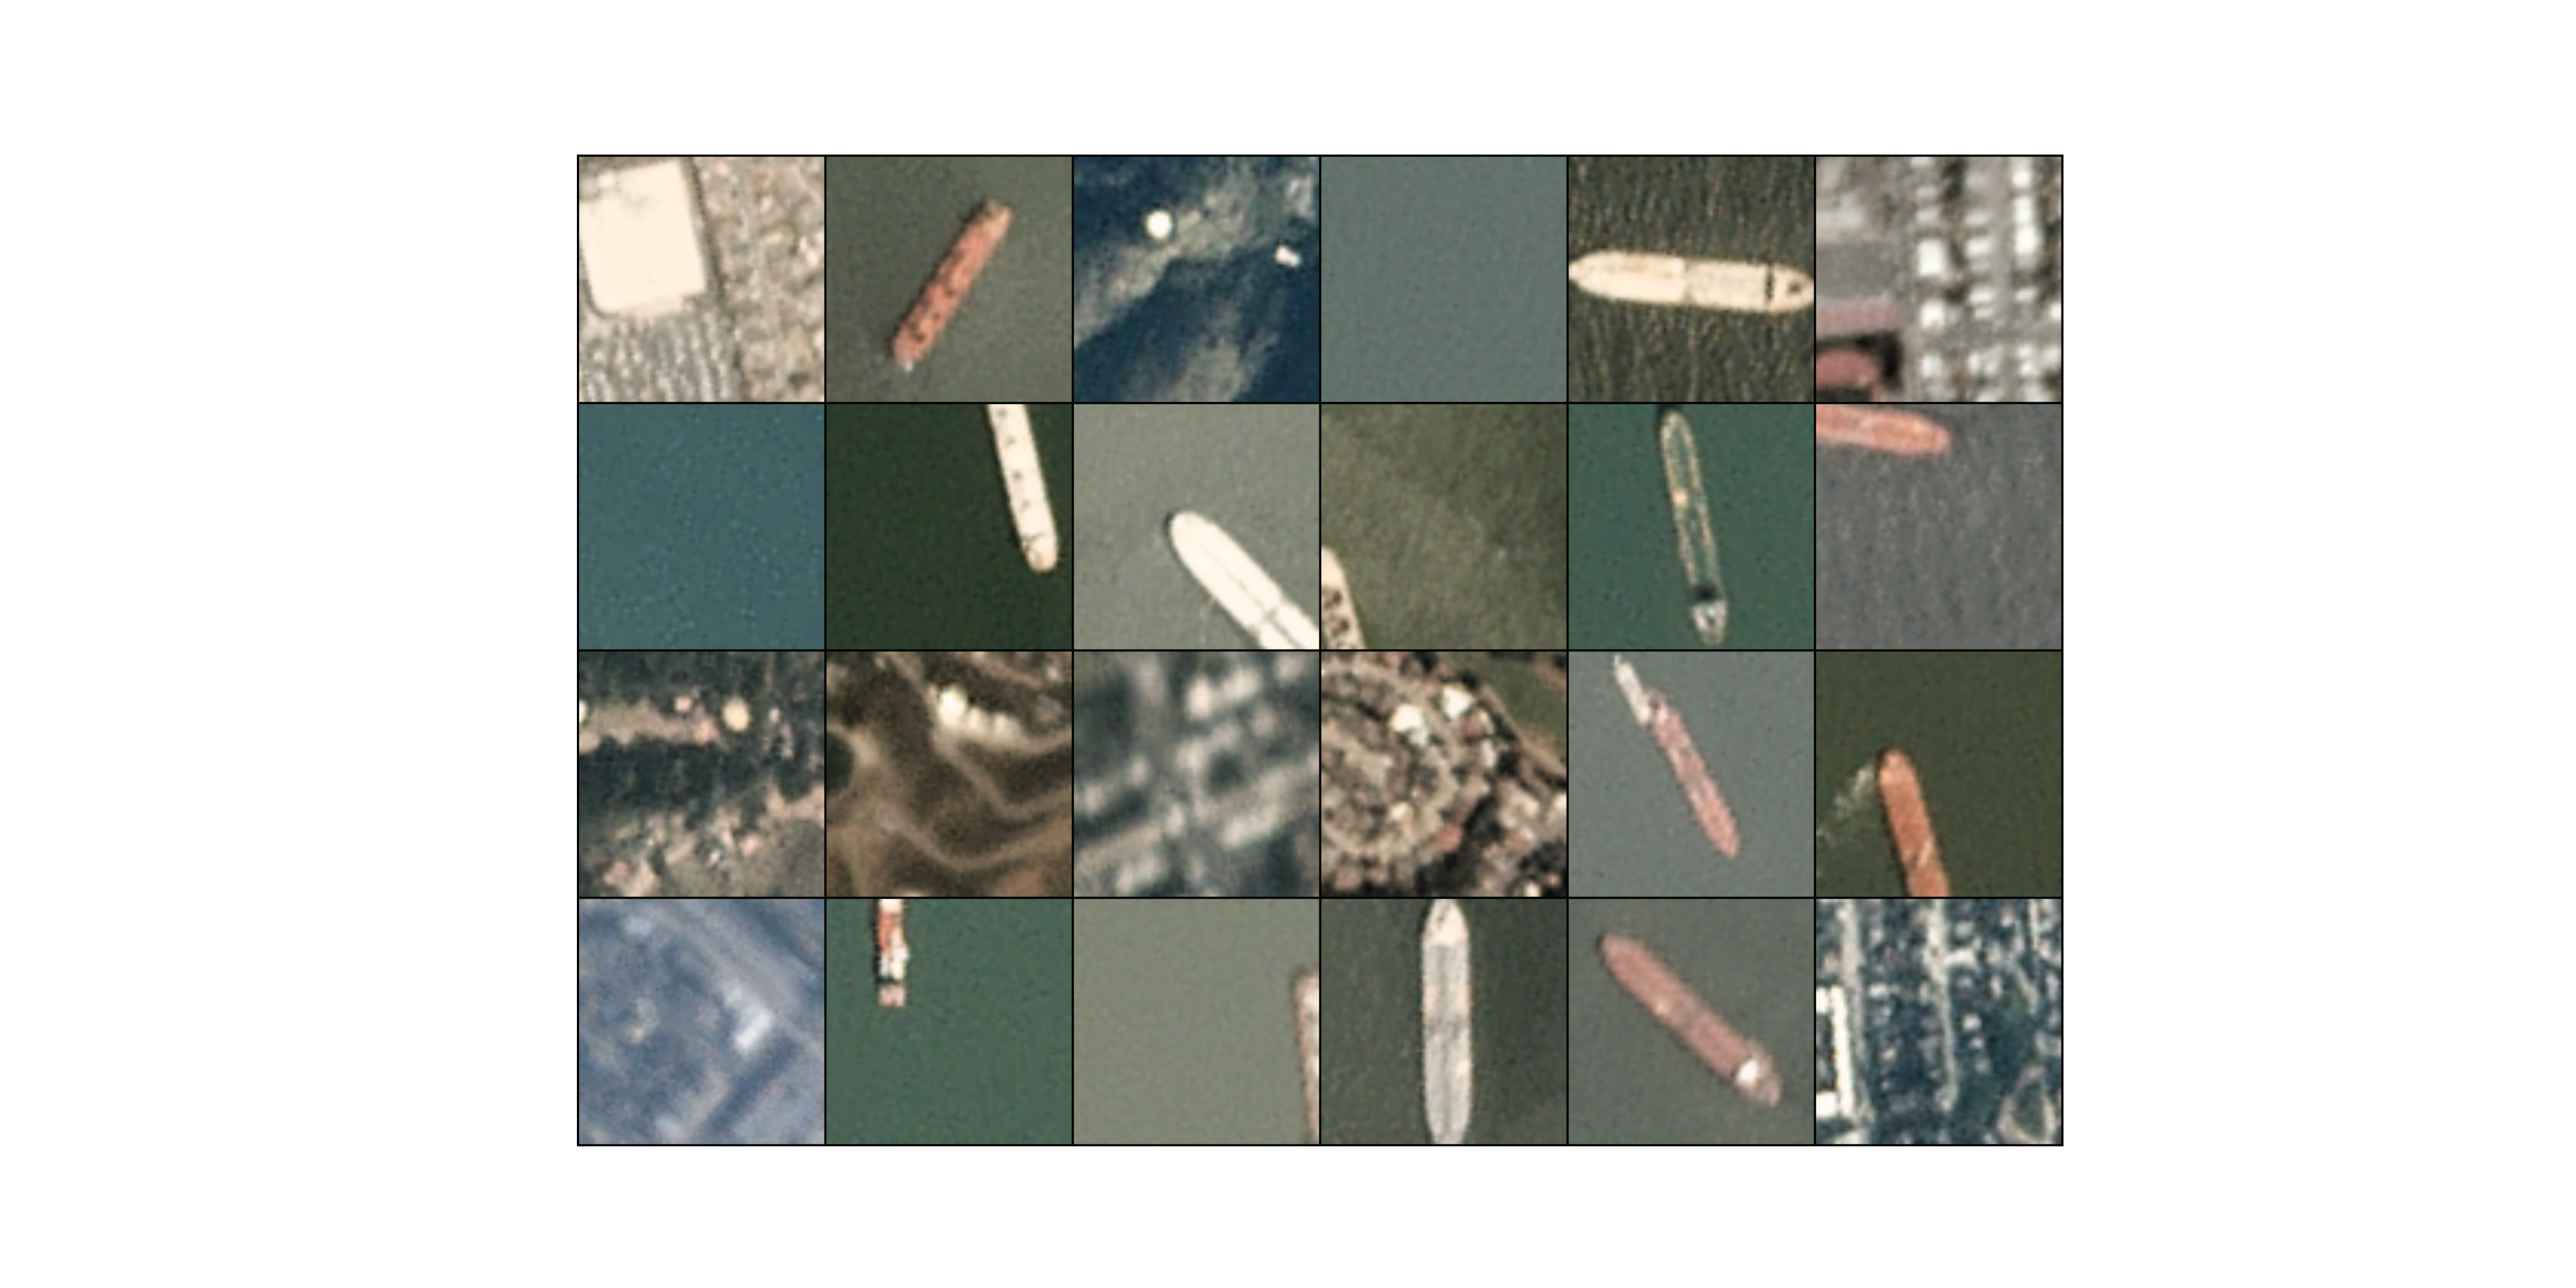
\includegraphics[width=\textwidth]{assets/vgg11_prediction_batch_grid.png}
%			\caption{VGG11}
%		\end{subfigure}
%		\hfill
%		\begin{subfigure}[b]{0.32\textwidth}
%			\centering
%			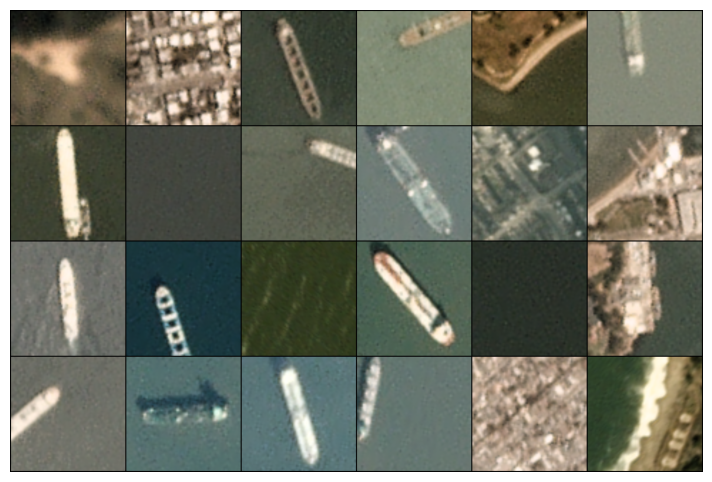
\includegraphics[width=\textwidth]{assets/resnet50_sample_predictions.png}
%			\caption{ResNet50}
%		\end{subfigure}
%		\hfill
%		\begin{subfigure}[b]{0\textwidth}
%			\centering
%			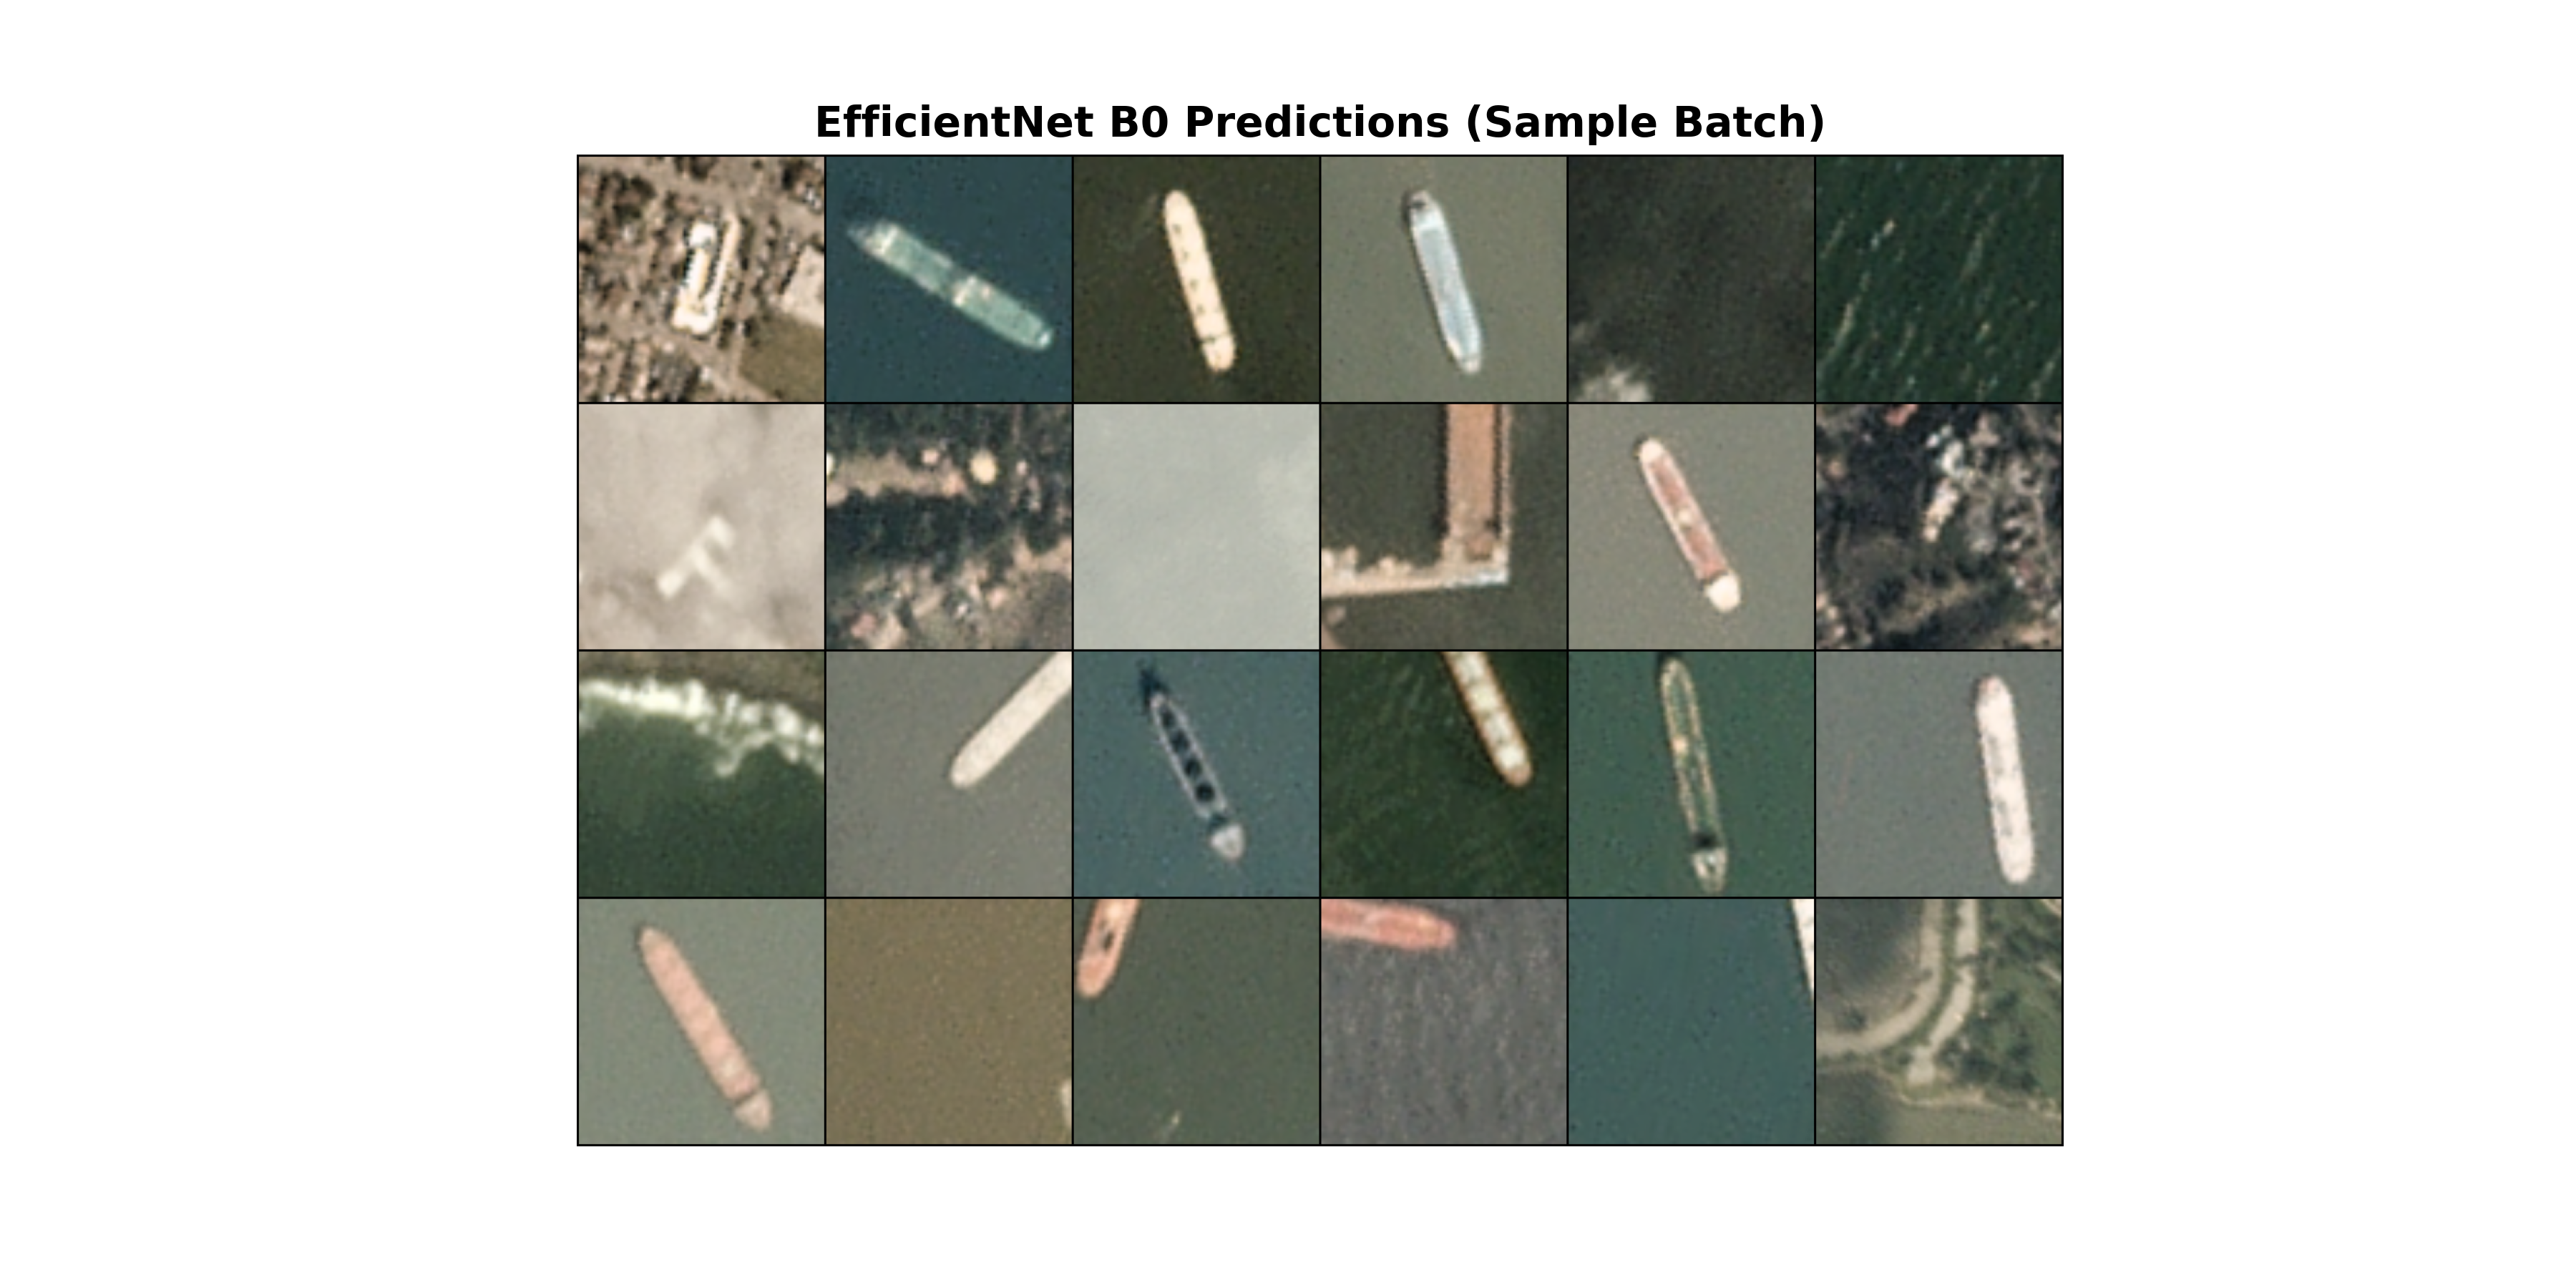
\includegraphics[width=\textwidth]{assets/effnet_b0_sample_predictions.png}
%			\caption{EfficientNet-B0}
%		\end{subfigure}
%		\caption{Sample Predictions}
%	\end{subfigure}
	
	
	\section*{Limitations}
	
	Observation of false positives. We observed some false alarms, mostly on features that resembled ships in size or colour. For instance, one image had a section of a pier that the model falsely highlighted (this is an example). This is likely due to the model's bias from the training set: many no-ship training chips contained ship-like elements, which can confuse the classifier.
	False positives could potentially be reduced by incorporating a water mask (so the model only scans areas known to be water)
	
	Window size constraint: using a fixed 80*80 window means the detector is tuned to ships of roughly that scale. If the ships in the scene is significantly larger than 80 pixels (e.g. a very large vessel) or much smaller, detection might be suboptimal. Our model requires the ship to mostly fit in the window to be confident. If the port image had ships larger than the chip size, the sliding window approach would still find them via multiple overlapping chips, but the model might see parts of a ship as "no-ship" if the ship is cut off. Advanced object detector would handle this via multi-scale feature maps
	
	Computation - sliding a window across an entire image is computationally expensive, though we mitigated it by batching predictions. A 3000 * 3000 pixel image would entail on the order of 9 million windows if done at every pixel - mention that using the GPU made this brute-force scanning feasible, but it won't scale well to very large or real-time use. Could further explore the use of YOLO.
	
	Environmental factors - note that our satellite images are optical (RGB) and presumably taken in clear conditions. The model would be challenged by clouds, extreme lighting changes, or if ships are camouflaged against backgrounds. Since it's trained on one specific port, it might not generalise perfectly to other ports without adaptation
	
	\section*{Conclusion}
	
	\newpage
	\begin{flushleft}
		\begin{thebibliography}{9}
			\bibitem{patel2022}
			Patel, K., Shah, J., Shah, M., and Shah, D.
			\textit{Deep Learning-Based Automatic Detection of Ships: An Experimental Study Using Satellite Images}.
			Journal of Imaging, 8(7), 2022.
			\url{https://doi.org/10.3390/jimaging8070182}
			
			\bibitem{rhammell2017}
			rhammell.\\
			\textit{GitHub - Rhammell/Shipsnet-Detector: Detect Container Ships in Planet Imagery Using Machine Learning}.\\
			GitHub, 2017.\\
			\url{https://github.com/rhammell/shipsnet-detector} (Accessed 27 Apr. 2025)
			
			\bibitem{zhao2024}
			Zhao, T., Wang, J., Li, Y., and Xie, H.\\
			\textit{Ship Detection with Deep Learning in Optical Remote-Sensing Images: A Survey of Challenges and Advances}.\\
			Remote Sensing, vol. 16, no. 7, 2024, pp. 1145--1145.\\
			\url{https://doi.org/10.3390/rs16071145} (Accessed 19 Aug. 2024)
			
		\end{thebibliography}
	\end{flushleft}
\end{document}